\documentclass{article}
\usepackage[utf8]{inputenc}
\usepackage[english]{babel}
\usepackage{amsmath}
\usepackage{amsfonts}
\usepackage{amssymb}
\usepackage{graphicx}
\usepackage{wrapfig}

\author{Arian Stolwijk}
\begin{document}

\section{Problem Description}

\begin{wrapfigure}{r}{0.4\textwidth}
  \vspace{-30pt}
  \begin{center}
    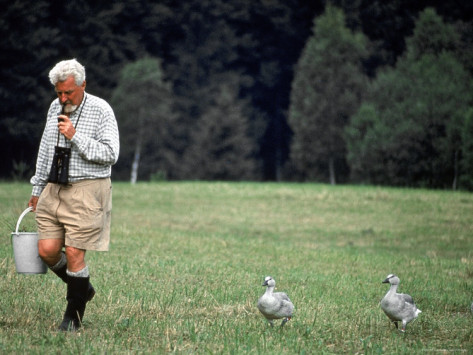
\includegraphics[width=0.38\textwidth]{geese.jpg}
    \vspace{-20pt}
  \end{center}
  \caption{Geese following a person}
  \label{fig:geese}
  \vspace{-20pt}
\end{wrapfigure}

When a goose comes out of their eggs, it assumes its mother to be the first
thing it sees. Usually this is true and then it follows the mother for ever.
However if this is a human, it will simply follow the human too, as seen in
figure~\ref{fig:geese}.

Using a smartphone and a simple robot we can simulate the same effect. The
smartphone as mother and the robot as baby goose. The objective of the robot is
to follow the smartphone.

\section{Sensors to be used}



\section{Theoretical methods to be used}

\section{Initial Results}

\end{document}

